\section{Filter design}
In this section the process of designing digital filters is described. There will be distinguished between techniques for IIR and FIR filters.\\ The section is concluded by a comparison of FIR and IIR filters.\\  
As described ideal filters are not computable. Hence the process of designing a filter is based on approximation of the frequency response - made by computable polynomials - based on a set of specification for the filter. There exist different design methods to achieve this.   
\subsection{IIR filter}
One common way of designing an IIR filter is to design the discrete-time filter from a corresponding continuous-time system. The method follows three main steps. 
\begin{itemize}
\item[1.] Specify the properties desired for the filter as filter specifications.
\item[2.] Hereby compute a "prototype" by a continuous-time system $H_c(\Omega)$ that approximates the given properties. In this rapport it is done as a \textit{Butterworth filter}.  
\item[3.] Transform the "prototype" into the discrete-time filter $H(\omega)$. In this rapport this is done with the \textit{Bilinear transformation}. 
\end{itemize}
The properties of a system are specified based on the desired application, considering what frequencies are to pass the filter ideally. Furthermore, it is important to specify how much the filter is allowed to vary from the ideal properties as an ideal filter is not a possibility. \\
Properties for an approximation to a lowpass filter is defined by bounding the amplitude within $\pm \ \delta_1$ of unity in a limited frequency band $0 \leq \Omega \leq \Omega_p $ and less than $\delta_2$ in the frequency band $\Omega_s \leq \Omega$. \\
The tolerance scheme based on the specifications of the continuous time filter is illustrated on figure \ref{fig:scheme}.
The transition of non zero width between the cut off frequency of passband and stopband is necessary in order for the system to be realizable.

\begin{figure}[H]
\centering
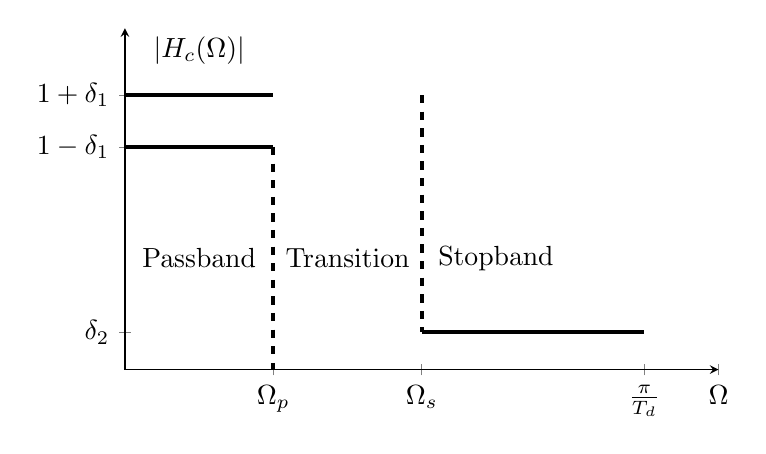
\begin{tikzpicture}[scale=1]
\begin{axis}[
scale=1.1,
unit vector ratio*=1 1 1,
axis lines = middle,
xtick={0,2,4,7,8},
xticklabels={$0$,$\Omega_p$,$\Omega_s$,$\frac{\pi}{T_d}$,$\Omega$},
ytick={0.5,3,3.7},
yticklabels={$\delta_2$,$1-\delta_1$,$1+\delta_1$},
xmin=0,
xmax=8,
ymin=0,
ymax=4.6]
\node at (axis cs:1,4.3) {$|H_c(\Omega)|$};
\draw[line width=0.5mm](axis cs:0,3.7)--(axis cs:2,3.7);
\draw[line width=0.5mm](axis cs:0,3)--(axis cs:2,3);
\draw[line width=0.5mm, dashed](axis cs:2,3)--(axis cs:2,0);
\draw[line width=0.5mm, dashed](axis cs:4,3.7)--(axis cs:4,0.5);
\draw[line width=0.5mm](axis cs:4,0.5)--(axis cs:7,0.5);
\node at (axis cs:1,1.5) {Passband};
\node at (axis cs:3,1.5) {Transition};
\node at (axis cs:5.0,1.5) {Stopband};
\end{axis}
\end{tikzpicture}
\caption{Specifications of amplitude response}
\label{fig:scheme}
\end{figure}

The predefined Butterworth filter is a lowpass filter approximation used to fit the filter to the requirements. For the Butterworth filter the squared amplitude response is defined as follows:
\begin{align}\label{eq:butter}
|H_c(\Omega)|^2=\frac{1}{1+\left( \frac{j\Omega}{j\Omega_c}\right)^{2N}}.
\end{align} 
Further the filter is characterised by the following three properties:
\begin{align}
1.& \ \ \ |H_c(\Omega)|^2 = 1 \  \ \left|\begin{matrix}
\\ 
\Omega=0
\end{matrix}\right. , \textit{ for all }N. \\
2.& \ \ \ |H_c(\Omega)|^2 = \frac{1}{2} \  \ \left|\begin{matrix}
\\ 
\Omega=\Omega_c
\end{matrix}\right. , \textit{ for all }N. \\
3.& \ \ \ \textit{Amplitude response is monotonic in pass- and stopband.}
\end{align}
As the order $N$ of the filter increases the characteristics become sharper and the filter approximates the ideal lowpass filter. This is illustrated on figure \ref{fig:butter}. By \eqref{eq:butter} it is possible to compute the order necessary for the system to fulfil the specifications.            
\begin{figure}[H]
    \centering
    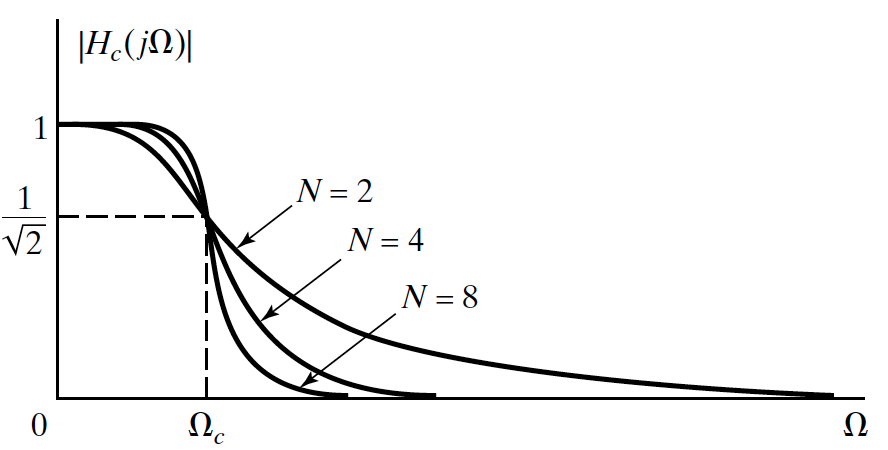
\includegraphics[width = 0.6\textwidth]{figures/butterworth.png}
    \caption{Magnitude of Butterworth filter depending on order $N$ }
    \label{fig:butter}
\end{figure} 
In order to obtain stability in the system representation in the $s$-domain is wanted. By substituting $s=j\Omega$ the following relation is true
\begin{align}
|H_c(s)|^2 = H_c(s)H_c(-s)= \frac{1}{1+\left( \frac{s}{j\Omega_c}\right)^{2N}}.
\end{align} 
By letting the denominator in \eqref{eq:butter} equal zero it is possible to determine the poles $s_k$ of the system
\begin{align}
1+\left( \frac{s}{j\Omega_c}\right)^{2N} = 0 \ \  \Rightarrow  \ \ \frac{s}{j \Omega_c} = \sqrt[2N]{-1} \ \
\Rightarrow 
\end{align}
\begin{align}
s_k = (-1)^{\frac{1}{2N}}\left(j\Omega_c\right)=\Omega_c\text{e}^{\left(\frac{j\pi}{2N}\right)\left(2k+N-1\right)}, \ \ k=0,1,\ ... \ , 2N-1.
\end{align}   
The poles will be placed equally along the circle of radius $\Omega_c$ in the $s$-plane. By only considering the poles in the left half plane, $H_c(s)$ can be construed as a stable system:
\begin{align}
H_c(s)=\frac{1}{\prod_{k=1}^{N}(s-s_k)}.
\end{align}    
When the continuous time filter $H_c(s)$ is defined the next step is the digitalization of the filter.  The Bilinear transformation is a method that allows a direct transformation between the s- and z-domain . The principal of the transformation is that the imaginary axis $j\Omega$ of the s-plane is mapped onto the z-plane as the unit circle. The bilinear transformation is defined by 
\begin{align}
s=\frac{2}{T_d}\left(\frac{1-z^{-1}}{1+z^{-1}}\right), 
\end{align}
such that 
\begin{align}
H_c\left[\frac{2}{T_d}\left(\frac{1-z^{-1}}{1+z^{-1}}\right)\right]=H_c(z). 
\end{align}  
Because $-\infty \leq \Omega \leq \infty $ is mapped to $-\pi \leq \omega \leq \pi$ the transformation most be non-linear which involves some frequency distortion. Because of this the method is restricted to situations where this is acceptable or can be compensated. Compensation can be done by the concept of prewarping, that uses the relation 
\begin{align}
\Omega_{c_{new}}=\frac{2}{T_d}\tan\frac{\omega_c}{2}.
\end{align}
Hereby it is possible to determine a new $\Omega_c$ to the continuous-time filter in order to ensure the discrete $\omega_c$ to fit the specification.\\
An important property of the bilinear transformation is that stability is preserved if the continuous-time filter i stable.
\subsection{FIR filter}\label{subsec:FIR}
Design of FIR filters are in contrast to IIR filters based on approximating the desired discrete-time frequency response directly. By this method it is possible to guarantee a general linear phase of the system. The method also uses the window method, which is described in the following section.
\subsubsection{The window method}
The window method is considered a simple method for designing FIR filters. The method takes off from the idealized desired frequency response $H_d$, defined to be equal to one in passbands and zero in stopbands corresponding to desired cutoff frequencies. Hereby the idealized impulse response $h_d[n]$ is obtained by the inverse Fourier transform of the desired frequency response
\begin{align}
h_d[n]=\frac{1}{2\pi}\int_{-\pi}^{\pi} H_d(\omega)\text{e}^{j\omega} d\omega.
\end{align}
$H_d(\omega)$ usually results in a impulse response of infinite length caused by the discontinuities at the boundaries between pass- and stopband. To compute a finite causal system as a FIR filter, on behalf of the desired impulse response $h_d[n]$, the realisable impulse response $h[n]$ of the FIR filter is determined as a product of the idealised impulse response $h_d[n]$ and a finite duration \textit{window} $w[n]$ 
\begin{align}
h[n]=h_d[n]w[n], \ \ w[n] =
\left\{ \begin{matrix}
f[n], &\ 0 \leq n \leq M \\
0, &\ Otherwise
\end{matrix}\right.
\end{align}

By this truncation the impulse response of a finite filter of order $M$ is determined such that
\begin{align}
h[n]= 
\left\{ \begin{matrix}
h_d[n]w[n], &\ 0 \leq n \leq M \\
0, &\ Otherwise
\end{matrix}\right.
\end{align}
This is illustrated by an example of the simple \textit{rectangular window} defined as 
\begin{align}
w[n] =
\left\{ \begin{matrix}
1, &\ 0 \leq n \leq M \\
0, &\ Otherwise
\end{matrix}\right.
\end{align}
By Fourier transformation this gives the following expression. Figure \ref{fig:rect_db} illustrates the main and side lobes by a decibel plot of the amplitude response corresponding to the rectangular window.
\begin{align}
W \left(\omega\right)=\sum_{n=0}^{M} \text{e}^{j\omega n} = \frac{1- \text{e}^{-j\omega(M+1)}}{1- \text{e}^{-j\omega}} = \text{e}^{-j\omega \frac{M}{2}} \frac{ \sin \left( \frac{\omega \left( M+1 \right)}{2} \right)}{\sin \left( \frac{\omega}{2} \right)}.
\end{align}

\begin{figure}[H]
\centering
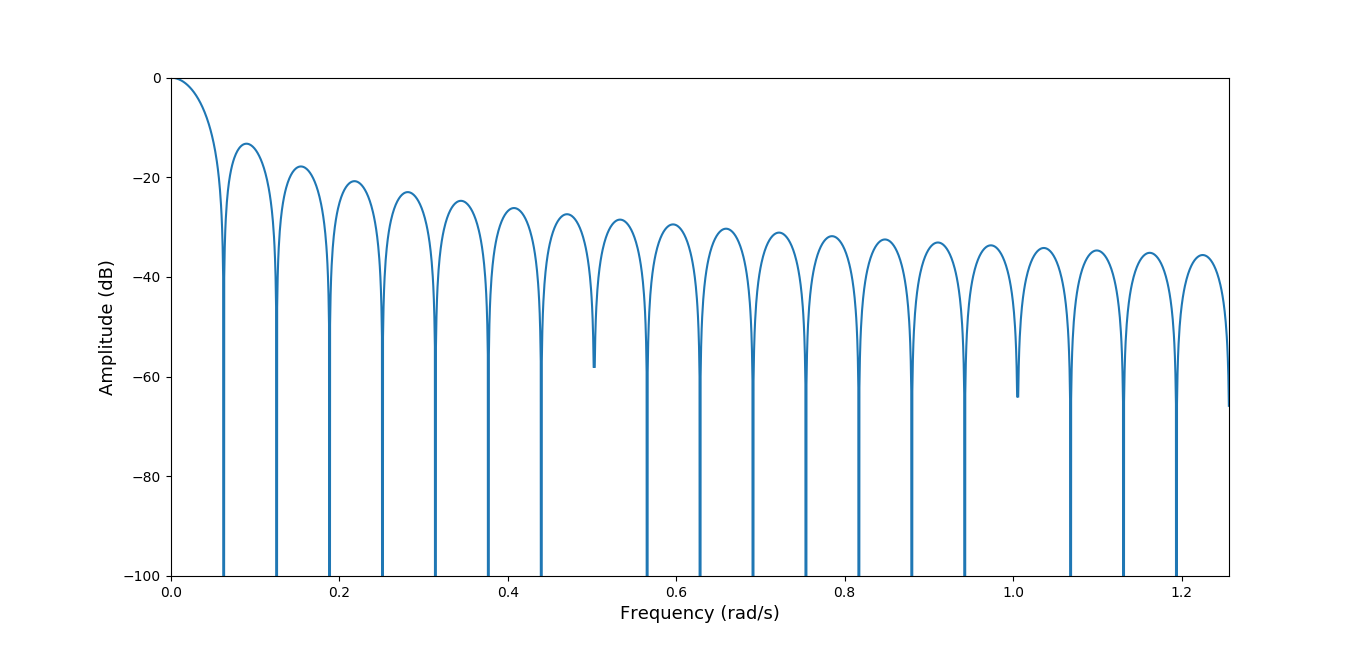
\includegraphics[width=\textwidth]{figures/dbplots/rect.png}
\caption{dB amplitude response of rectangular window of order $M=100$.}
\label{fig:rect_db}
\end{figure}

%
%\begin{figure}[H]
%\centering
%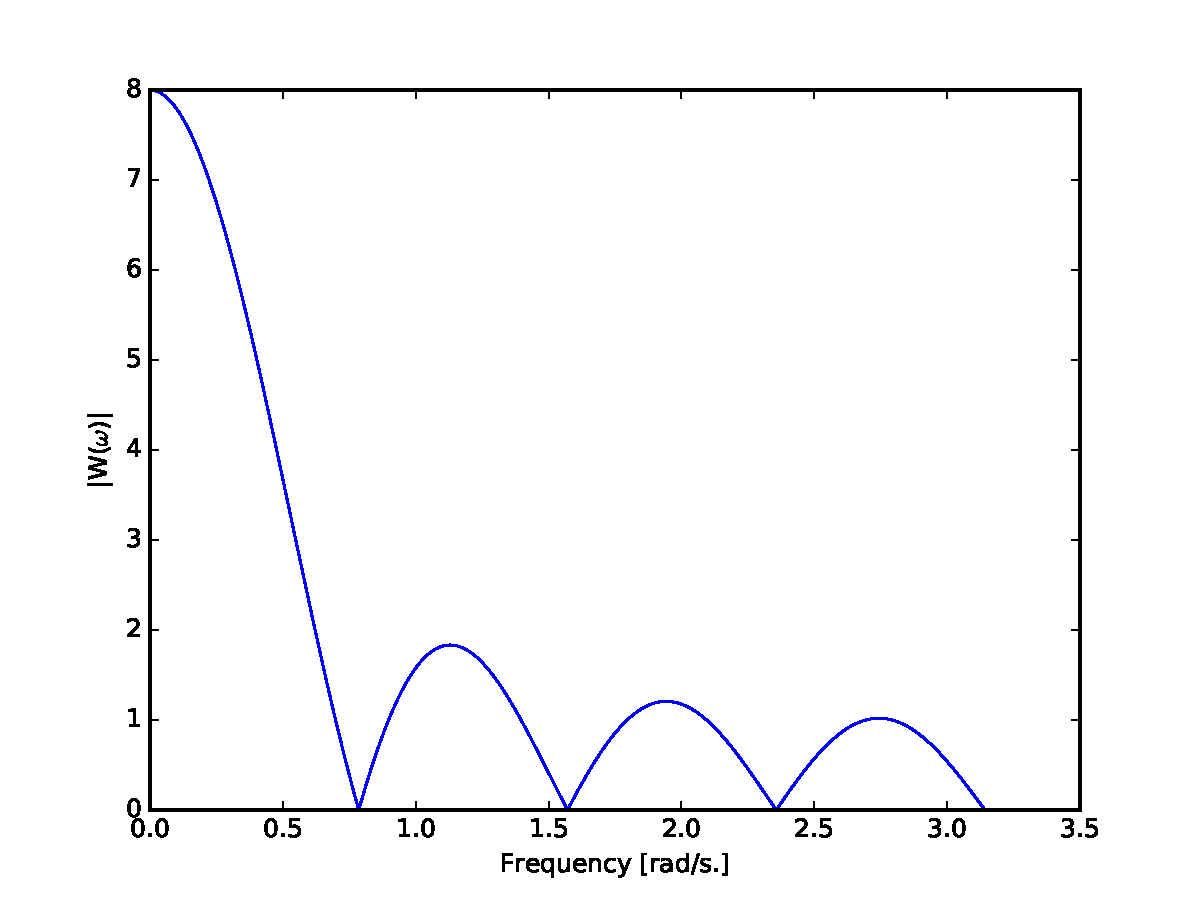
\includegraphics[scale=0.4]{figures/filter_teori/W_rect.pdf}
%\caption{Absolute amplitude response of the rectangular window of order $M=8$.}
%\label{fig:W_rect}
%\end{figure}
The aim is to approximate the desired frequency response as good as possible. For $w[n]=1 \ \forall \ n$, $W(\omega)$ becomes a periodic impulse, which implies that $H(\omega) = H_d(\omega)$ though the needed truncations are not performed. The impulse train is best approximated by letting the main lobe of $W(\omega)$ be as narrow as possible and the side lobes as small as possible. This corresponds respectively to minimizing the width of the transitionband and the ripples in pass- and stopband, though it is not possible to achieve both at ones.\\
By increasing the filter order $M$, the width of the main lope is decreased, but the peak amplitude of the side lopes also increases, which results in ripples. This indicates a trade-off between the width of the main lope and the amplitude of the side lopes. \\

\subsubsection{Different types of windows}
The rectangular window is one out of many windows that have different properties. The oscillations in the $H(\omega)$ is a result of Gibbs phenomenon. According to convergence of Fourier series this can be improved by convolving the desired frequency response with a less abrupt window. By narrowing each end of the rectangle smoothly towards zero, the amplitude peak of the side lopes are remarkably decreased, though this will still result in a wider main lope. \\
In table \ref{tab:window} some commonly used windows are defined. Furthermore, the windows and the corresponding amplitude response in dB of three different windows are illustrated by figure \ref{fig:windows}.
\begin{table}[H]\small
\centering
\caption{Definition of different types of windows}
\label{tab:window}
\begin{tabular}{l|l} \hline
Rectangular & $w[n] =
\left\{ \begin{matrix}
1, &\ 0 \leq n \leq M \\
0, &\ Otherwise
\end{matrix}\right. $ \\ \hline
Bartlett    & $w[n] =
\left\{ \begin{matrix}
\frac{2n}{M}, &\ 0 \leq n \leq \frac{M}{2} \\
2-\frac{2n}{M}, &\ \frac{M}{2} \leq n \leq M \\
0, &\ Otherwise
\end{matrix}\right.$ \\ \hline
Hanning     & $w[n] =
\left\{ \begin{matrix}
0.5-0.5 \cos(\frac{2\pi n}{M}), &\ 0 \leq n \leq M \\
0, &\ Otherwise
\end{matrix}\right. $ \\ \hline
Hamming     & $w[n] =
\left\{ \begin{matrix}
0.54-0.46 \cos(\frac{2\pi n}{M}), &\ 0 \leq n \leq M \\
0, &\ Otherwise
\end{matrix}\right. $ \\ \hline
Blackman    &  $w[n] =
\left\{ \begin{matrix}
0.42-0.5 \cos(\frac{2\pi n}{M}) + 0.08 \cos(\frac{4\pi n}{M}), &\ 0 \leq n \leq M \\
0, &\ Otherwise
\end{matrix}\right.$  \\ \hline
\end{tabular}
\end{table}    

\begin{figure}[H]
\centering
\begin{subfigure}{0.49\textwidth}
\centering
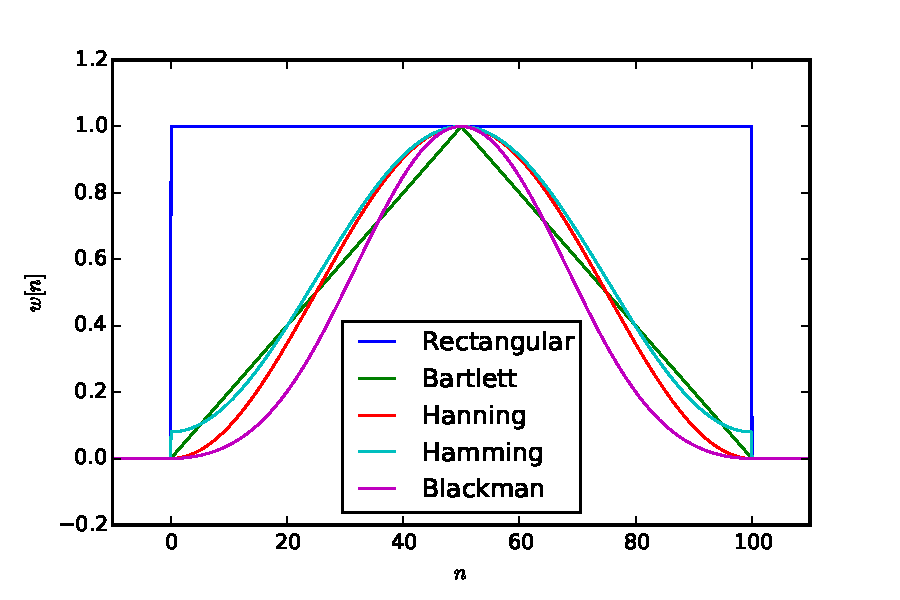
\includegraphics[width=\textwidth]{figures/filter_teori/window_types.pdf}
\caption{Window functions in time domain}
\label{fig:win_type}
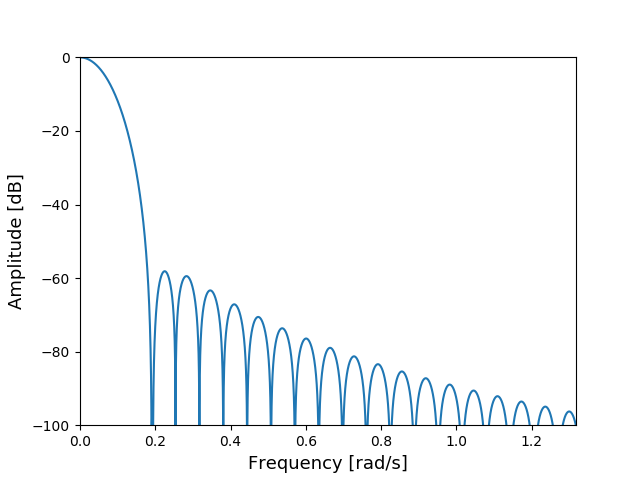
\includegraphics[width=\textwidth]{figures/dbplots/blackman.png}
\caption{Blackman}
\label{fig:blackman_db}
\end{subfigure}
\begin{subfigure}{0.49\textwidth}
\centering
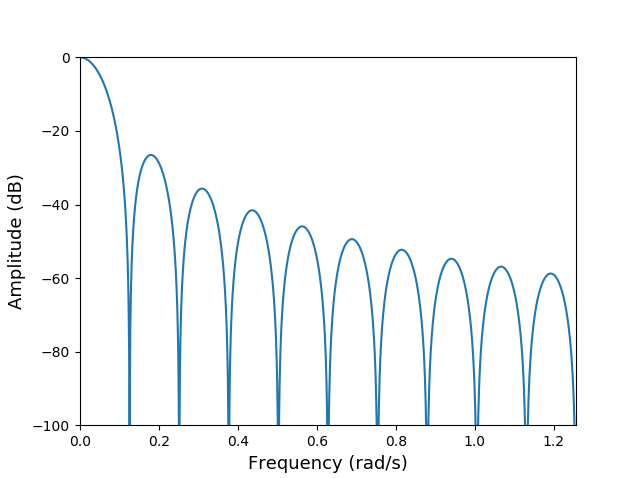
\includegraphics[width=\textwidth]{figures/dbplots/bartlett.png}
\caption{Hann}
\label{fig:hann_db}
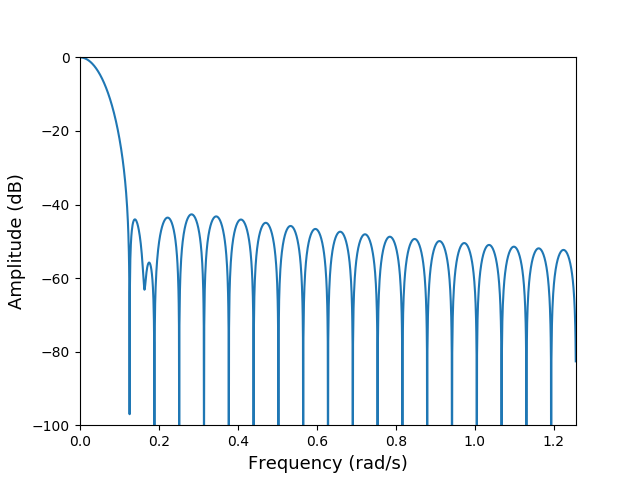
\includegraphics[width=\textwidth]{figures/dbplots/hamming.png}
\caption{Hamming}
\label{fig:hamming_db}
\end{subfigure}
\caption{(a) Different window functions in time domain of order $M=100$ (b, c, d) dB amplitude of frequency response of chosen windows of order $M=100$.}
\label{fig:windows}
\end{figure}

The defined windows all have the property of being symmetric around the point $\frac{M}{2}$. Hence, if the ideal impulse response is also symmetric the windowed impulse will be symmetric, which results in a frequency response with generalized linear phase. \\
To conclude this section it is seen that in order to design a FIR filter by the window method one can vary the chosen window and the order of the system until the desired specifications are achieved.

\subsubsection{The Kaiser window method}
The Kaiser window design method considers the Kaiser window as the near-optimal window which - compared to the other windows - has two parameters; the length $M+1$ and a shape parameter $\beta$. This results in \textit{one} window where changing the parameters adjusts shape and length of the window in order to achieve the optimal trade-off between amplitude of side lopes and width of main lope. The Kaiser window is defined as 
\begin{align}
w[n]=\left\{\begin{matrix}
 \frac{I_0[\beta (1-[\frac{n-\alpha}{\alpha}]^2)^{\frac{1}{2}}]}{I_0(\beta)} , &\ 0 \leq n \leq M  \\ 
0, &\ \text{Otherwise}
\end{matrix}\right.
\end{align}

where $\alpha=\frac{M}{2}$ and $I_0(\cdot)$ is the zero'th order modified Bessel function of the first kind \cite{DTSP, page 474-476}. Increasing $\beta$ tapers the window in the time domain, which results in smaller side lopes of the Fourier transform. Increasing $M$ causes the width of the main lope to increase but without changing the peak amplitude of the side lopes. This is illustrated in figures \ref{fig:kaiser_beta} and \ref{fig:kaiser_order}, respectively.\\

\begin{figure}[H]
\centering
\begin{minipage}{0.49\textwidth}
\centering
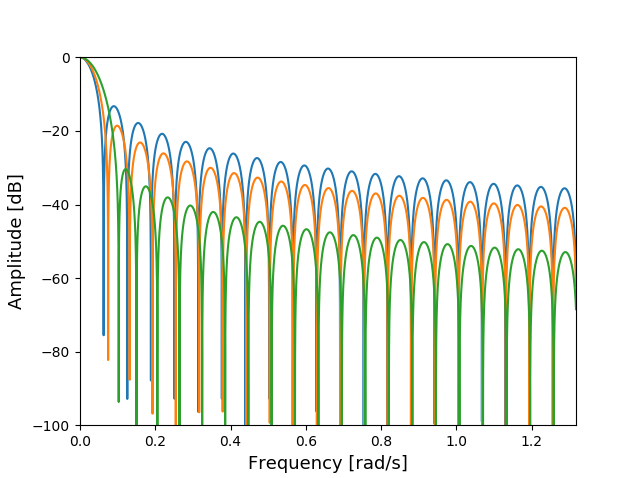
\includegraphics[width=\textwidth]{figures/dbplots/kaiser_beta.png}
\caption{dB amplitude response of Kaiser windows of order $M=100$ with $\beta=0,2$ and 4 for blue, orange and green respectively. As $\beta$ increases the side lobes become smaller.}
\label{fig:kaiser_beta}
\end{minipage}
\begin{minipage}{0.49\textwidth}
\centering
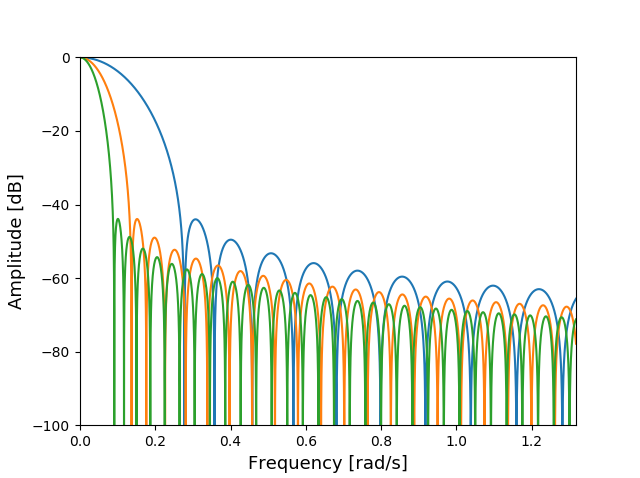
\includegraphics[width=\textwidth]{figures/dbplots/kaiser_order.png}
\caption{dB amplitude response of Kaiser windows with $\beta=6$ and order $M=50,100$ and 150 for blue, orange and green respectively. As $M$ increases the main lobe becomes narrower.}
\label{fig:kaiser_order}
\end{minipage}
\end{figure}
 
In order to determine values for $\beta$ and $M$ according to  satisfying the desired specifications the following formulas are defined. Considering a lowpass filter with a fixed peak approximation error $\delta$ this gives a cutoff frequency of the passband $\omega_p$ defined by $|H(\omega)| \geq 1-\delta$ and cutoff frequency of the stopband $\omega_s$ defined by $|H(\omega)| \leq \delta$. This gives a transitionband of width $\Delta \omega = \omega_s - \omega_p$. Defining $\delta$ in $[dB]$ by $A=-20\log_{10} \delta$ it is possible to determine the value of $\beta$ on behalf of a specific value of $A$ as 
\begin{align}
\beta =
\left\{ \begin{matrix}
0.1102\left( A-8.7 \right), &\ A \geq 50 \\
0.5843\left(A-21\right)^{0.4}+0.07886(A-21), &\ 21 \leq A \leq 50 \\
0.0, &\  A \leq 21 
\end{matrix}\right.
\end{align}
       
Furthermore, $M$ must satisfy the following relation:
\begin{align}
M=\frac{A-8}{2.285\Delta \omega}.
\end{align}

By this establishment of the Kaiser window method it is possible to design a FIR filter within desired specifications with almost no iterations or trial and error. By adjusting the shape parameter $\beta$ it is possible to obtain a window equivalent to each of the windows defined in table \ref{tab:window} with a more narrow transition width, which could make the Kaiser window preferable.       
   
\subsection{Comparison of IIR and FIR filters}
This section about the design of digital filters concludes with a comparison of IIR and FIR filters, which considers the advantages and disadvantages of the different systems. \\ 
\\
The process of designing an IIR filter - presented in this section - is rather simple when the desired properties fits a predefined filter such as a Butterworth filter. The required order of the filter is computable, and the transformation to the discrete time domain is done straight forward. Furthermore, considering the implementation, this leads to a recursive algorithm. By this method the magnitude response is the only parameter to be specified, hence specific requirements for e.g. phase response or group delay are not guaranteed to be fulfilled by this kind of IIR filter. \\ \\
Considering a FIR filter the main advantages - compared to IIR filters - is the possibility of getting a precise generalized linear phase. The generalised linear phase is important in order to preserve the wave form of the original signal.  
The window method is also straight forward to apply, though it is not pre-defined design equation, and so more or less iterations are often necessary before desired specifications are achieved. \\
When choosing the right filter design computational speed is often considered, which basically is related to the required order of the system and amount of needed iterations. \\
\\
By this it is clear that the choice of filter depends on the specific case and how different aspects are weighted. IIR filters have many advantages in implementation and efficiency which makes it preferable in cases, where the need of generalized linear phase is less significant, but in other cases linear phase by a FIR filter can be worth the extra computations.